\documentclass{cmspaper}

\newcommand {\ie}{\mbox{\sl i.e. }}     %i.e.
\newcommand {\eg}{\mbox{\sl e.g. }}     %e.g.


\begin{document}

%==============================================================================
% title page for few authors

\begin{titlepage}

% select one of the following and type in the proper number:
%   \cmsnote{2005/000}
  \internalnote{2005/XYZ}
%  \conferencereport{2005/000}
   \date{\today}
\smallskip
\smallskip
 \rightline{\bf Version 0.1}


  \title{Requirements and Design of the Physics and Data Quality
Monitoring infrastructure at CMS}

  \begin{Authlist}
    C.~Leonidopoulos and E.~Meschi
       \Instfoot{cern}{CERN, Geneva, Switzerland}
  \end{Authlist}

% if needed, use the following:
%\collaboration{Flying Saucers Investigation Group}
%\collaboration{CMS collaboration}

  \begin{abstract}
  This note describes the set of requirements and the architecture of
the Physics and Data Quality Monitoring framework. 
  \end{abstract} 

% if needed, use the following:
%\conference{Presented at {\it Physics Rumours}, Coconut Island, April 1, 2005}
%\submitted{Submitted to {\it Physics Rumours}}
%\note{Preliminary version}
  
\end{titlepage}

\setcounter{page}{2}%JPP

%==========================================
\section{Introduction} \label{sec:introduction}
%==========================================
%
The Physics and Data Quality Monitoring framework (DQM) aims at
providing a homogeneous monitoring environment across various
applications related to data taking at CMS. It must be fairly flexible
and easily customizable so it can be used by different groups across the
experiment. Examples of ``customers'' that can benefit from a common monitoring
package are: the high-level trigger algorithms in the Filter Farm,
subdetector groups that wish to supervise the operation of local DAQ
systems, or even purely off-line batch jobs in a potentially
``production validation'' scheme. 

The DQM organizes the information received by a number of monitoring
producers and redirects it to monitoring-consuming clients according to their
subscription requests (see Fig.~\ref{fig:generic_diagram} for a
generic graphical representation of the producer-client
relationship). On the producer side, it uses an implementation-neutral
interface allowing direct insertion of monitoring statements in the
reconstruction code. This interface can be accessed from standalone
programs, or can be used from within \eg ORCA ``applications'' and
``modules''. On the client side, an interface connects the received
objects with a set of tools for evaluating the monitoring information,
setting alarms and accessing a monitoring database for storing objects
and editing log files.
%
\begin{figure}[hbtp]
  \begin{center}
  \rotatebox{90}{
    \resizebox{17cm}{!}
	{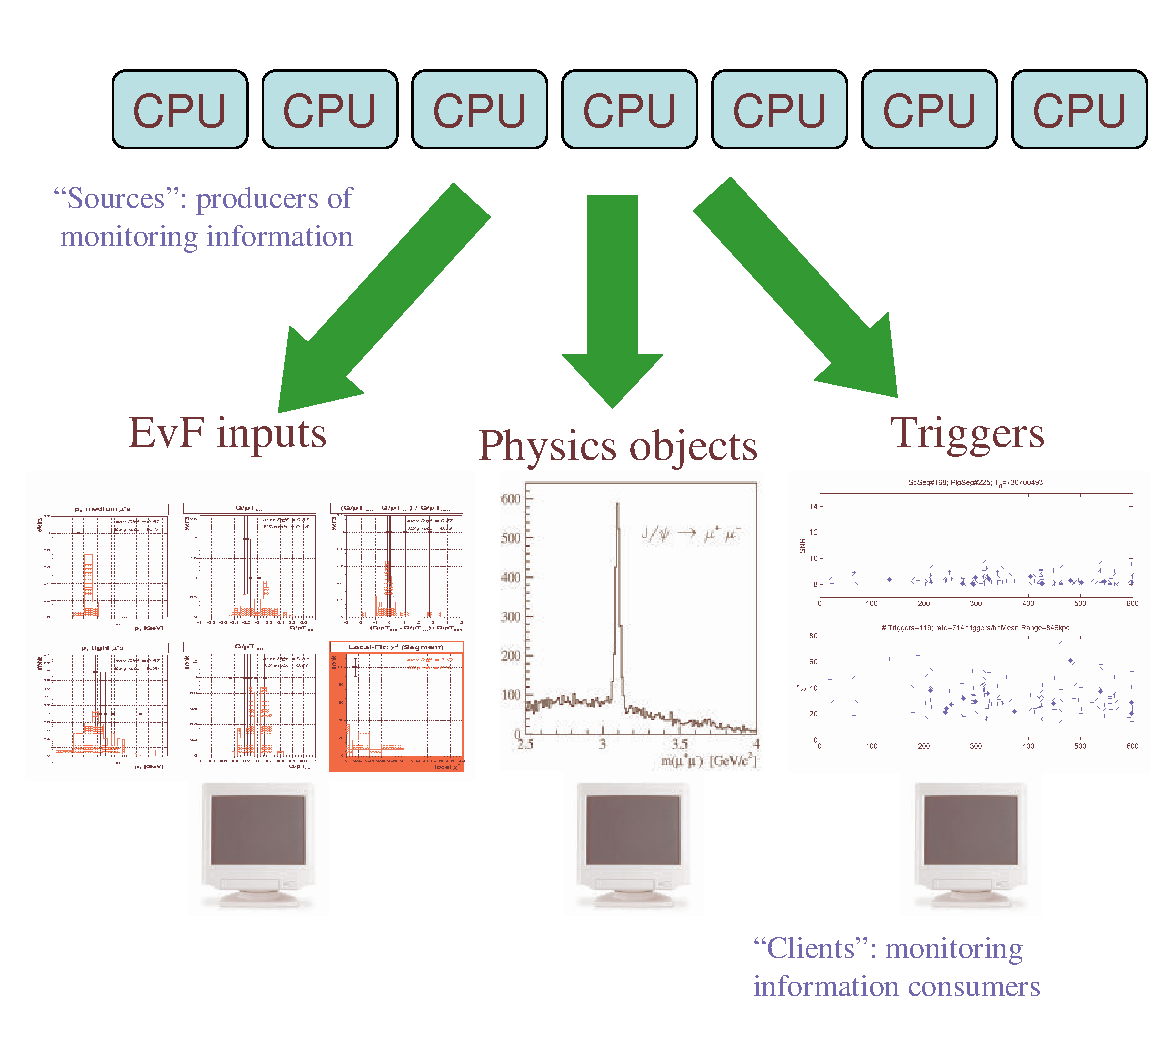
\includegraphics{figures/generic_diagram.eps}} }
\caption{DQM is a generic monitoring framework serving different customers.}
\label{fig:generic_diagram}
  \end{center}
\end{figure}
%%
%
%
%==========================================
\section{General} \label{sec:general}
%==========================================
%
The DQM is designed to receive sets of objects (``monitoring elements'', or ME)
from monitoring producers (``sources''), organize and
redistribute them on a periodical basis. Sources are defined as
individual nodes that have either direct access to or can process and
produce information we are interested in. The creation and update of
MEs at the source can be the result of processing input event data
(event consumers) or input monitor elements (monitor consumers).

At the other end of this architecture are the monitoring information
consumers (``clients'') that receive a list with the available monitoring
information (``monitorable'') from all sources combined. The clients can
subscribe to and receive periodic updates for any desired subset of the
monitorable, in a classic implementation of the ``publish-subscribe'' service.

We introduce a hierarchical system of nodes that are responsible for
the communication between sources and clients (\eg subscription
requests) and the actual monitoring transfer. These nodes serve as
collectors for the sources and as monitoring servers for the clients,
and will be called ``collectors'' in the rest of this document.

For small monitoring systems, a single collector should be
sufficient (Figure ~\ref{fig:single_collector}). For larger systems
(\eg the HLT Farm), one could envisage different levels of merging
and elaboration. For example, in Figure ~\ref{fig:multiple_collectors}
a first level of collectors is responsible for gathering all the
monitoring information from multiple sources, effectively sharing the
bandwidth and the workload. A second level of collectors is used to
sort the monitoring already gathered according to content. A client
could connect to one or more collectors, depending on the kind of
information it is interested in subscribing.
%
\begin{figure}[hbtp]
  \begin{center}
    \resizebox{10cm}{!}
	{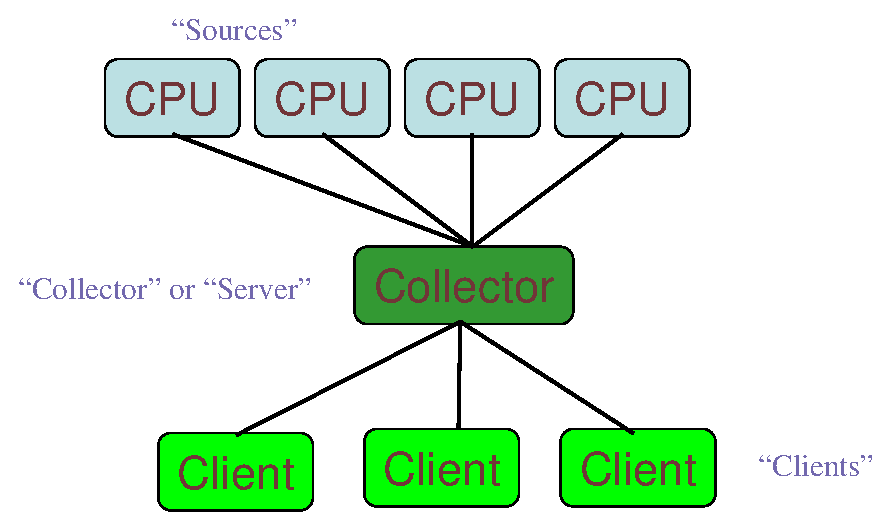
\includegraphics{figures/single_collector.eps}} 
\caption{A simple monitoring system with a single collector.}
\label{fig:single_collector}
  \end{center}
\end{figure}
%
\begin{figure}[hbtp]
  \begin{center}
    \resizebox{13cm}{!}
	{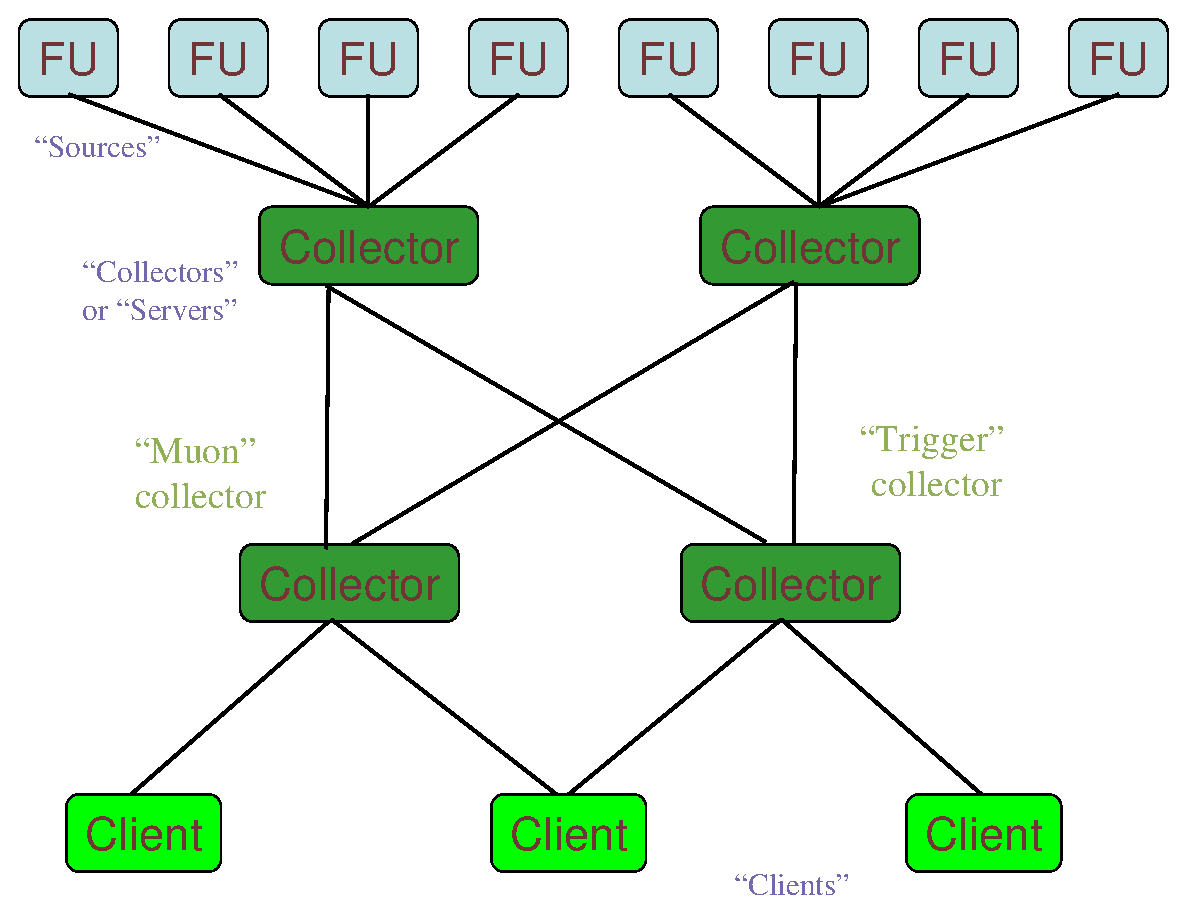
\includegraphics{figures/multiple_collectors.eps}} 
\caption{The high-level trigger farm as an example of a more complex monitoring
system with two levels of collectors needed.}
\label{fig:multiple_collectors}
  \end{center}
\end{figure}
%
The collector ``hierarchy'', namely the full network of nodes that connects a
source to the client and the exact configuration of its members, is
static. It is never modified after startup. The configuration should
clearly define the ``coupling point'' (\ie collector) that  every
source and client can connect to. Whereas source and clients should be
able to disconnect and reconnect at run-time (\ie without affecting the
stability of the rest of the system), the collector network
must be always running if the monitoring service is meant to be uninterrupted.

A decision has been made that the DQM process should do the minimum
necessary work at the source level. This is simply an attempt to minimize the
interference with the ``main'' application running at the source
node (\eg analysis, calibration/alignment, trigger algorithm,
etc). To that end, sources are connected to only one collector each
(but a collector can connect to multiple sources). Clients do not have
direct access to the sources. All source-client communication is done
through the collector (or collectors). 

All CPU-intensive tasks (\eg comparison to reference monitoring
element, display, database storage, etc.) should be attached at the client's
side. 

This designs aims at
%
\begin{itemize}
\item{shielding the sources from connecting clients
that could slow down the main application or threaten the stability of
the source, and}
\item{facilitating the quick transfer of the monitoring
information from the sources to the collectors.} 
\end{itemize}
%
The production of the monitoring information is clearly separated from
the collection and the processing. The collectors act as the ``middle
man'': they are responsible for advertising the monitorable to
different clients and serve monitoring requests.

In normal running mode, sources and clients are in an infinite
monitoring loop:
%
\begin{itemize}
\item{
The source task list consists of 
\begin{itemize}
\item{sending the full monitorable to the collector once (and updates,
when necessary)}
\item{receiving (un)subscription requests (if any), and}
\item{sending the udpdated monitoring information to the collector}
\end{itemize}
}
\item{
The client task list consists of 
\begin{itemize}
\item{receiving the monitorable from all sources when connecting
(including updates, when necessary)}
\item{(un)subscribing to a(ny) subset of the available monitoring
information}
\item{receiving the updated monitoring information, and}
\item{performing operations on MEs, setting alarms,
accessing the monitoring database (see below)}
\end{itemize}
}
\end{itemize}
%
%
%==========================================
\section{Limitations}\label{sec:limitations}
%==========================================
%
The nature of the collection and processing of the monitoring
information is statistical by construction. In particular, the DQM 
\begin{itemize}
\item{is meant to help the experts identify problems that occur (and monitored)
\emph{over a period of time}. }
{\item does \emph{not} give access to particular events.}
%types footnote{Insofar as the
%sources do not have access to ??? event types. Sources can work off a
%specific DAQ live on hot buffer, which is fed by selected particular events
%out of a miselected(?) stream.}
{\item does \emph{not} guarantee that two clients will receive identical
monitoring information.}
\end{itemize}
%
The monitoring cycle\footnote{Defined as the time between two consecutive
shipments of the updated MEs from the source to the
collector (for the source), or from the collector to the client (for
the client).} may not be constant in time, especially for monitoring
configurations in which the shipping time is comparable to the requested
update period. Furthermore, the DQM should have the flexibility to
dynamically adjust the monitoring rate, or even skip monitoring
cycles, in order to minimize deadtime. The skipped monitoring packages
are not considered lost information, as long as the exact fraction of
the monitoring cycles received by the client is known.
%
%==========================================
\section{Requirements}\label{sec:requirements}
%==========================================
%
\subsection{General}
\label{sec:req_general}
The DQM provides support for 
\begin{itemize}
\item{storing monitoring information into 1D-, 2D- and 3D-histograms,
profiles, scalars (integer and real numbers) and string messages. It
does \emph{not} provide support for full events, raw data or other
objects\footnote{This is provided by an independent mechanism, not
discussed here.} that cannot be accomodated in one of the above formats.} 
\item{abstract interfaces for booking, filling and MEs (see Appendix,
Sec.~\ref{app:neutral_interface} for the rationale of this choice).}
\item{directory structures, \ie unix-like directories with
virtually unlimited depth, from which the monitoring client can ``pick
and choose'' (Fig.~\ref{fig:dir_structure_support}). }
\item{creation of root-tuples with the monitoring structure ``on demand''.}
\item{\emph{dynamic} lists of sources and clients: individual sources and
clients can be added or removed at run-time.} 
\end{itemize}
%
\begin{figure}[hbtp]
  \begin{center}
    \resizebox{10cm}{!}
	{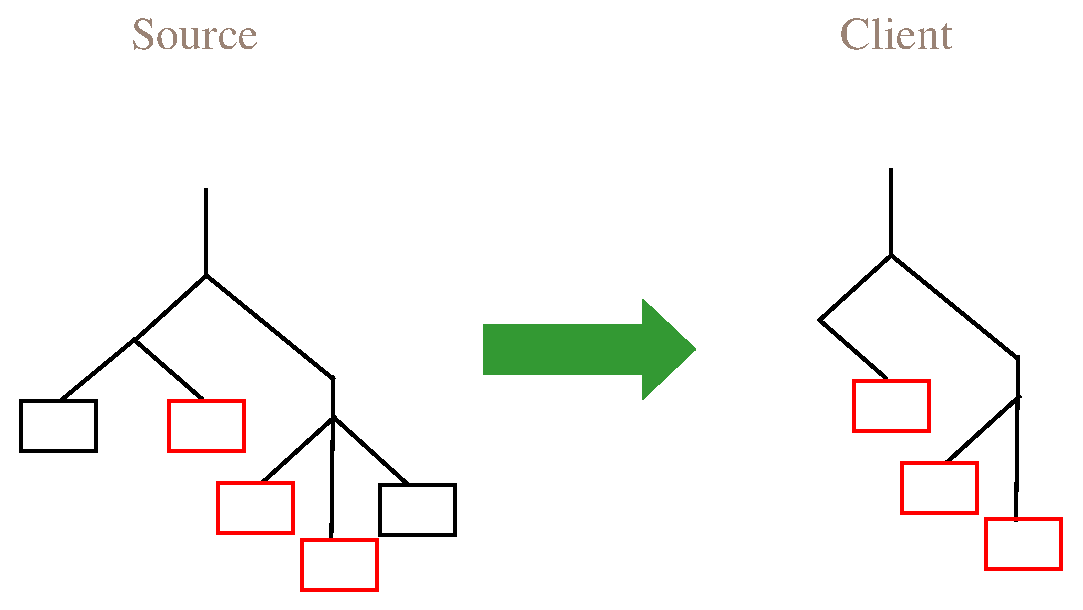
\includegraphics{figures/dir_structure_support.eps}} 
\caption{DQM support for directory structures and subscription ``\`a
la carte''.}
\label{fig:dir_structure_support}
  \end{center}
\end{figure}
%
%
\subsection{Sources}
\label{sec:req_sources}
\begin{itemize}
\item{Support for \emph{static} monitorables (\ie monitorables defined
at start-up).}
\item{Support for \emph{dynamic} monitorables: the sources should be able to
update the list of available monitoring information at run-time and
advertise it to the monitoring clients (through the collectors).}
\item{The sources need not do more than booking and filling (and potentially
deleting) MEs. The framework takes care of
communicating this information to the client.}
\item{Stability: the main application should not be affected if the connection
with the collector is lost (\eg the collector has crashed).}
\item{Support for a ``reset'' switch specifying whether monitoring
contents should be reset at the end of monitoring cycle. This flag (defined per
ME) should be {\tt true} for MEs that describe dynamic content (\eg hit
occupancy of a subdetector) and {\tt false} for MEs that describe
accumulating quantities (\eg \# of events processed, \# of fatal
errors caught, or rare counters).}
\end{itemize}
%
%
\subsection{Clients}
\label{sec:req_clients}
\begin{itemize}
\item{The clients should be able to receive monitoring information
from multiple sources.} 
\item{Support for reception of static and dynamic monitorables from all
sources (\ie ``initial'' list of MEs at startup, and
subsequent updates if necessary).}
\item{Support for static monitoring subscription lists (\ie automatic
loading and transmission of a subscription list, as well as ``edit''
and ``save'' functionality).}
\item{Support for dynamic monitoring subscription lists: the clients
should be able to subscribe and unsubcribe at run-time ``\`a la carte''.}
\item{The clients should be able to request additional monitoring
information (not listed in the initial monitorable). This would be
equivalent to a ``debug'' command that requests the creation of an
extra (temporary) set of MEs from one or more
sources. At some subsequent time, the client is expected to issue
another command cancelling the request (instructing the sources to
cease producing the extra monitoring information, and therefore, lower
the monitoring load).} 
\item{Support for a user interface that provides access to a set of
tools (discussed in Sec.~\ref{sec:tools}).}
\item{Stability: the main application should not be affected if the connection
with the collector is lost (\eg the collector has crashed).}
\end{itemize}
%
%
\subsection{Collectors}
\label{sec:req_collectors}
\begin{itemize}
\item{Support for dynamic lists of sources and clients: A collector
should be able to handle 
\begin{itemize}
\item{disconnecting or dying nodes (sources and
clients), as well as}
\item{new connections at run-time.}
\end{itemize}
Every time the number of active nodes changes, the collector must
modify monitorable and subscription requests accordingly.}
\end{itemize}
%
%
\subsection{Client tools}
\label{sec:tools}
%
As discussed in Sec.~\ref{sec:general}, the majority of the operations
or tasks involving MEs takes place on the client side. Here we define
a set of tools used for these tasks, accessible only by clients.
%
\subsubsection{Analysis tools for monitoring element operations}
\label{sec:analysis_tools}
%
\begin{itemize}
\item{``Soft'' reset: operation that resets the contents of a ME 
for $t < t_0$ (the user should still have access to both $t < t_0$ and
$t > t_0$ intervals). This functionality is useful only for MEs
with the ``reset'' switch set to {\tt false} (specified at the source, see
Sec.~\ref{sec:req_sources}).}

\item{``Accumulate'': operation that sums the contents of a ME
 over many monitoring cycles. This functionality is useful only
for MEs with the reset switch set to {\tt true} (specified at
the source)}.

\item{Collation: sum up MEs at client's side: 
$$C \equiv \sum_i h_i $$
where $h_i$ is the $i^{\rm th}$ ME and $C$ the sum of all MEs.

It is the client's responsibility to make sure that the resulting ``summary''
ME makes sense (\ie collation of identical-in-format
MEs).}

\item{``Hard'' reset: In addition to the ``soft'' reset functionality, the
user has the option of permanently erasing the contents of ME that has
been defined locally (and is therefore invisible to other nodes), \eg
an ``accumulation''- or ``collation''-type ME.}

\item{Comparison to reference ME: \eg Kolmogorov's test (giving the ``\% C.L.''
that a histogram and its reference are consistent with each other),
``\# of sigmas away from expected value'', etc.}

\end{itemize}
%
%
\subsubsection{Alarm class}
\label{sec:alarm_class}
The overall ``status'' of a ME can, for display purposes, be
summarized by a single discrete parameter. This is convenient for
summary pages on a GUI that can give the overall status of a
subdetector with a color-coded system. For example, the list of
warning types (and associated color on the display) could include
\begin{itemize}
\item{``New'': a new alarm has appeared (red).}
\item{``Acknowledged'': an alarm has been acknowledged; action still pending
(orange).}
\item{``Addressed'': the problem still remains, but experts have been
notified or a plan has been made (yellow).}
\item{``No warning'': no problem exists (green).}
\end{itemize}
%
The user is able to set, raise or lower alarms according to
information extracted with the tools described in
Sec.~\ref{sec:analysis_tools}. The alarm setting can be manual,
automatic or hybrid. This aims at accomodating different situations,
such as commissioning periods, routine problem-checking and cases
where either a program or the user can make the call.
%
%
\subsubsection{Monitoring database and archiving capabilities}
\label{sec:monitoring_database}
Users should be able to store (and retrieve) custom sets of MEs. The
user interface should provide
\begin{itemize}
\item{Support for various sets of MEs: ``current'' (\eg last
hour, day, week) or ``older'' (\eg last run, month or year).} 
\item{Option for storing objects on a server (``official'') or
locally.}
\item{Access to ``reference'' sets (determined by trigger configuration:
\ie. luminosity, trigger streams, prescales, etc).}
\item{Support for configuration lists for DQM clients (\eg. default
subscription lists, update frequencies, etc).}
\item{Access to a ``problem and solution'' history. Quering flexibility is
desired (\eg per subdetector and/or per run, week or with
any other ``keyword'').}
\end{itemize}
%
%
\subsubsection{Control structure and configuration}
\label{sec:control_structure}
\begin{itemize}
\item{The infrastructure supports the concept of a DQM configuration
containing the list of DQM processes that must be configured  for normal
data taking.}
\item{Each application can be started centrally and constantly
reports its status to a supervising entity.}
\item{Each application exposes a control interface similar to one used to
control the DAQ system. This interface is used  by the DAQ supervisor(s) to
control the operation of the various processes. The interface can be
customized to allow direct interaction with an individual DQM process to
perform specific  operation via a UI.}
\end{itemize}
%
A hypothetical task list here could include
\begin{itemize}
\item{configuring and starting a DQM process.}
\item{displaying a report on the DQM process status.}
\item{an interface \`a la ``run control'' for automated actions
(\eg stop- and start-run, reset, reconfigure).}
\end{itemize}
%
%
\subsubsection{Display and Graphical User Interface}
A GUI gives users a quick way of accessing the UI methods discussed in
this section. A non-exhaustive list includes
\begin{itemize}
\item{Global display with individual tabs per group (giving a ``one button''
access to the state of all subdetectors: warnings, \# of processed
events, rates, etc).}
\item{Option for static display or cycling through subscription list.}
\item{Navigation capability: browse though monitoring structure and click
on desired ME.}
\item{Web-based display client.}
\end{itemize}
%
The GUI would ideally be easily customizable, to allow different
groups to tailor it to their needs. An investigation of different
software packages is currently underway for selecting a
suitable application development framework.
%
%
%================
% Appendix
%================
\newpage
\appendix 
\bigskip

\section{Rationale for accessing monitoring elements via a neutral interface}
% that does not depend on a specific implementation:
\label{app:neutral_interface}
The current implementation of the monitoring transfer mechanism from a node to
another involves {\tt ROOT} (classes {\tt TSockets}, {\tt
TServerSocket} and {\tt TMessages}). This is out of convenience, since
users have expressed the desire to be able to save monitoring
structures in root-tuples that they can access later. Since the
``behind-the-scenes'' mechanics is implemented with {\tt ROOT}, one 
would be tempted to allow users to deal directly with {\tt ROOT}
objects. However, we have made the choice to hide the ``true'' format
behind a transparent interface for both sources and clients, for a
variety of reasons:
\begin{itemize}
\item{An abstract interface does not bind the user access methods to a
specific analysis framework and/or implementation. In our particular
case, the transfer mechanism and the ``true''
ME format ({\tt ROOT}) could change in the future, without
breaking the source and client programs.}
\item{Having an abstract interface that hides the raw monitoring data from
the user is a good OO practice. The set of allowed operations on the
monitoring objects should be defined by the (abstract) user interface,
not the framework used for the implementation.}
\item{Additional functionality can be added to the monitoring objects
(\eg alarms) without directly inheriting from {\tt ROOT} classes.}
\end{itemize}


\end{document}
